
\documentclass[11pt,a4paper]{report}
\usepackage{amsmath}                    % Extended math options
\usepackage{amssymb}                    % For special symbols, like collections Z,Q,R, etc.
\usepackage{epsfig}                     % To handle .eps figures


\setlength{\parindent}{0cm}             % No indent at first line of paragraphs
\renewcommand{\baselinestretch}{1.2} 	% More spacing between lines

% Differential operator
\newcommand{\diff}{\ensuremath{\mathrm{d}}} 

% Super and subscript
\newcommand{\supsc}[1]{\ensuremath{^{\text{#1}}}}   % Superscript in text
\newcommand{\subsc}[1]{\ensuremath{_{\text{#1}}}}   % Subscript in text

\newcommand{\vt}[1]{\ensuremath{\boldsymbol{#1}}} % vector in correct lettertype
\newcommand{\mx}[1]{\ensuremath{\mathsf{#1}}}	  % matrix in correct lettertype

\newcommand{\omex}{\boldsymbol{\omega}_x}


\newcommand{\firstauth}[2]{\vspace{-\bibsepup}{\sc #1{,} #2}} %
\newcommand{\auth}[2]{{\sc #1{,} #2}} % use comment as \auth{Luppes}{R.}
\newcommand{\bibc}{{,} }              % separation between authors; no space!
\newcommand{\biba}{ and }             % last separation between authors
\newcommand{\noopsort}[1]{}           % correct bibliography order wrt year
\newlength{\bibsepup}                 % bibitems a bit higher \bibsepup;
\setlength{\bibsepup}{2.0mm}          % prevents too much spacing
\newcommand{\etal}{et al.}            % xspace would give too much space !

% End of the preamble.
% Beginning of body:

% Special word splittings
\hyphenation{back-slash}
\hyphenation{split-sings-uit-zon-de-ring}

\title{Tea with a Travelling Salesman:\\
	\large A Discussion of Genetic Algorithms}
\author{Karin Dijkstra, Anastasia Dryaeva, Rick Ploeg \& Oliver Strik\\
Propaedeutic Project: A11\\
Rijksuniversiteit Groningen}
\date{June 6 2017}
 

\begin{document}

\maketitle

\begin{abstract}
Abstract needs to be copied here!
\end{abstract}

\tableofcontents

% The various chapters
%\newpage 
\section{Introduction}

\par
The Travelling Salesman Problem (TSP) is a famous problem in combinatorial optimization, with the goal to minimize the total travel cost (be that time, distance, or fuel expenses) for a salesman who has to visit a finite number of cities and return to the starting point, given the costs associated with travelling from one city to another.

\par
At first the problem may appear uncomplicated and straightforward, however its simplicity is only an illusion. Although the exact origins of the TSP are unclear, it can be dated back to at least 1832, yet to this day, there has been no effective solution method found for a general case. In fact, a solution of this problem would resolve the infamous P vs. NP Millennium Prize problem. As a result, the Travelling Salesman Problem still remains one of the most intensely studied problems in computational mathematics and in the recent years has sparked interests in newer fields, such as computer science.

\par
Throughout the years, different methods and algorithms have been developed for the TSP. Many of the traditional methods involve heuristics such as Nearest Neighbor or Nearest Insertion, or relaxations, for example the Hungarian Algorithm. However, these do not necessarily give the optimal, and for the latter sometimes not even a feasible solution. Moreover, these methods become insufficient when the problem takes a larger scale. An example of a more advanced, newer method would be the application of a Genetic Algorithm. Genetic Algorithms (GAs) are algorithms designed to simulate natural evolution: they are based on the concept of “survival of the fittest”.

\par
This article will address the topic of applying a Genetic Algorithm to the Travelling Salesman Problem, focusing on the following question: “How do Genetic Algorithms perform when applied to the Travelling Salesman Problem?”. In order to provide an answer to this question, the TSP will be discussed in more detail in section \ref{IntroTSP}. After that, the general concept of a GA will be explained in section \ref{WisGA}, including an insight into the construction of such an algorithm for the TSP. In section \ref{SimpleTSP} the constructed GA will be applied to a small problem of 6 cities, where the efficiency of the algorithm will be evaluated in comparison to the traditional methods. Section \ref{largeTSP} will focus on investigating the performance of the GA on an expanded problem of 26 cities, including a discussion of the issues encountered, followed by a detailed analysis of the parameters within the constructed GA in section \ref{Analysis}. In the final section conclusions will be made, addressing the initial research question.




\chapter{What is a Genetic Algorithm}
%\input{How does the Genetic Algorithm perform on a simple TSP?}
\chapter{How does the GA perform on a TSP of a larger scale?}
\section{Introduction}

\par
Considering the characteristics of a Genetic Algorithm, one can assume that they are not the standard method to use on problems of such a small scale as the problem discussed in Chapter 2, since manual or traditional methods can give the solution as well. GAs hold their real value in problems of a larger scale. Here they are capable of giving a feasible solution, where most other methods fail to give one or are just highly inefficient. The constructed GA has proved itself capable of dealing with a simple TSP containing six cities, but how does it perform on a TSP of a larger scale? This chapter will discuss the answer to that question, explaining the obstacles encountered along the way.

\par
The details of the TSP, such as the number of cities and their locations, will be addressed in the next section of this chapter. Then in the third section, the first performance of the GA on this TSP will be discussed. Since the total of possible tours was relatively low for the simple TSP, discussed in the previous chapter, the GA was capable of finding the optimal tour in every run. In this larger TSP however, the number of tours is significantly larger, which meant that the GA did not find the optimal tour in every run. This problem is known as premature convergence and is the topic of the fourth section. In the last section of this chapter a possible method to prevent premature convergence is discussed.

\section{A TSP containing 26 cities}
For this expansion it was decided to extend the problem to 26 cities. To make the problem more realistic, these 26 cities were selected to be located throughout the Netherlands. 

\begin{table} [t]
\parbox{0.4\textwidth}{

\begin{tabular}{l}
1 Amersfoort\\ 
2 Amsterdam\\
3 Apeldoorn\\
4 Arnhem\\
5 Assen\\
6 Breda\\
7 Den Haag\\
8 Den Helder\\
9 Eindhoven\\
10 Emmen\\
11 Enschede\\
12 Groningen\\
13 Haarlem\\
14 Heerenveen\\
15 Heerlen\\
16 ‘s-Hertogenbosch\\
17 Leeuwarden\\
18 Lelystad\\
19 Maastricht\\
20 Middelburg\\
21 Nijmegen\\
22 Rotterdam\\
23 Tilburg\\
24 Utrecht\\
25 Venlo\\
26 Zwolle
\end{tabular}

\label{26cities}
}
\qquad
\begin{minipage}[c]{0.6\textwidth} 
\footnotesize
\centering
\graphicspath{ {Afbeeldingen/} }
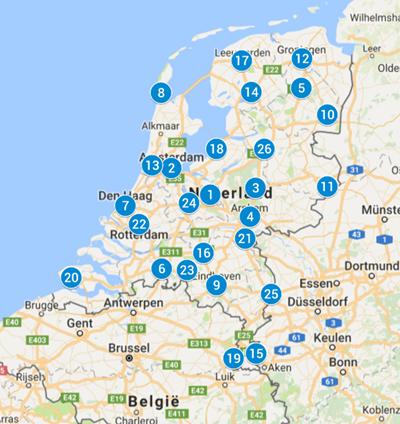
\includegraphics[width=1.2\textwidth, center]{26cities}
\captionof{figure}{26 cities, marked on the map of the Netherlands}
\label{map1}
\end{minipage}
\end{table}

\newpage
\par
The 26 cities are listed in alphabetical order together with a map of the Netherlands (figure \ref{map1}), that marks all of their locations. The objective is thus to find the shortest route that visits all of these cities and returns to the starting point afterwards. The total number of possible tours here is calculated by equation: %future reference needed
\[n = \frac{(26-1)!}{2} =  7.755605e+24\]
This number is significantly larger than the 60 possible tours for the simple TSP, discussed in chapter 2. This is then also the reason why most other methods fail to give a solution or are just inefficient. The manual methods and traditional methods, discussed in the previous chapter, are excellent examples. The Hungarian Algorithm already took 2 hours to perform on a TSP, containing only six cities and even though it did give the optimal solution in the end, it is highly inefficient to apply to this TSP because of the time it would take. In addition, this algorithm is a manual method, which makes it susceptible for human errors. The BIP also fails to give a solution, because the number of integer variables exceeds the limit of the Microsoft Excel linear solver. Even without this limit of variables, a BIP would take a long time to construct, considering all the possible subtours that would have to be added to the program as constraints in order to make sure that the resulting tour meets the criteria, set by the TSP. All of these subtours have to be excluded by manually adding these constraints, which makes the BIP timewise an inefficient method.Therefore it is necessary to turn to other methods, such as Genetic Algorithms. Even though they are not bound to give the optimal solution, they are at least capable of giving a suitable tour that meets the criteria, set by the TSP.

\section{The performance of the GA}

\par
The first observation, when the GA was applied to the expanded TSP, was that the time for one run of the program had increased. Depending on the settings, such as the number of generations and the poolsize, the program now takes approximately a minute. Since one chromosome now consists of not 6, but 26 genes, it makes sense that the time for one run increased. One minute is still a relatively short amount of time to find a solution. Besides the short time, another benefit is that the GA did not need reconstructing in order to be applied to this expanded TSP. Because of the way the basic structure was programmed, this GA can be applied to any TSP, that sparks your interest given that you provide the necessary data, which consists of the number of cities and their distances to each other. For other methods, like the Hungarian Algorithm or the BIP, this does not hold. 

%\input{Analysis}
%\input{Discussion, issues, further research and conclusion}
%\begin{thebibliography}{9}
\bibitem{Google}
Google.
\textit{Google Maps} [Google Maps distances].
Retrieved: May 19, 2017.

\bibitem{Congress}
L. Juan, C. Zixing, and L. Jianqin.
"Premature convergence in genetic algorithm: Analysis and prevention based on chaos operator."
\textit{Proceedings of the 3rd World Congress on Intelligent Control and Automation} 2010: 495-499.

\bibitem{Popdiv}
Y. Leung, Y. Gao, and Z. Xu.
"Degree of Population Diversity - a Perspective on Premature Convergence in Genetic Algorithms and Its Markov Chain Analysis." \textit{IEEE Transactions on Neural Networks}, 8(5) (1997): 1165-176. 

\bibitem{Operations}
J.D.C. Little, K.G. Murty, D.W. Sweeney and C. Karel. "An algorithm for the traveling salesman problem." \textit{Operations Research}, Vol. 11 (1963): 972–989.

\bibitem{Basics}
M. Mitchell.
\textit{ An introduction to genetic algorithms.} Cambridge MA: MIT Press, 1998.

\bibitem{Premconvergence}
H. M. Pandey, A. Chadhary and D. Mehrota.
"A Comparative Review of Approaches to Prevent Premature Convergence in GA." \textit{Applied Soft Computing} 24 (2014): 1047-1077. 

\bibitem{Online}
D. Pardini.
[\textit{TSP optimum tour}], November 9 2015. Retrieved: June 5, 2017. Available: https://otimizacaonapratica.wordpress.com/2015/11/09/o-problema-do-caixeiro-viajante/.

\bibitem{populationsize}
B.R. Rajakumar and Aloysius George. "APOGA: An Adaptive Population Pool Size Based Genetic Algorithm." \textit{AASRI Procedia} 4 (2013): 288-96.

\bibitem{Thesis}
J. P. Ryan.
\textit{An algorithm for the solution of a traveling salesman problem to minimize the average time to demand satisfaction} [Unpublished master's thesis]. Texas AM University, 1992. Retrieved: June 3, 2017.
\end{thebibliography}




\end{document}

